\section{Architecture}
Before diving into the code and its structure, let's take the time to understand how the developers worked. Before \doom, everything had been done on a PC. Code was written, compiler compiled and the executable was started on the same machine. With the introduction of \NeXT workstations in the toolchain, things had to be different.\\
\par
A developer had two machines, a \NeXT workstation and a PC. All work was done on the \NeXT. Code was written with \cw{TextEdit.app}, compiled with \cw{gcc}, linked with \cw{ld} and tested there. The biggest advantage of working on an Unix system was stability. Developer never lost their work because the IDE crashed\footnote{With Borland C++, crashes were a daily occurrence.}.\\
\par
Once the developer was happy with the result, he switched to his second machine. In order to do so, he literally rolled his chair to the PC where the \NeXT workstation hard-drive was mounted over NFS. On this side, the PC compiled the same source code\footnote{With some platform specifics.} using \cw{WATCOM.EXE}, linked with \cw{WLINK.EXE} which generated \cw{DOOM.EXE}. \\
\par
 In this setup the PC was relegated to "only" running the game and assessing performances. The PC hard-drive was actually used only to boot the machine and host \cw{WATCOM} compiler. Everything else including \cw{DOOM.EXE} executable was stored on the \NeXT SCSI HDD.\\
\par
There were significant obstacle to this methodology. First of all, DOS programs had direct access to the hardware whereas NeXT process had to use "official" APIs. Second and perhaps most importantly, the two machines had different endianess. PCs ran on Intel CPUs which were little-endian whereas \NeXT were using Motorola 68040 CPU which were big-endian.\\
\vspace{2mm}
\par
\begin{figure}[H]
\centering
\scaleddrawing{0.8}{dev_setup}{Next HDD user home folder is mounted on DOS machine as Z drive.}
\end{figure}
\par



\subsection{Endianness}
Endianness was a term introduced by Danny Cohen in his essay "On holy wars and a plea for peace". His satire, based on Gulliver's Travels in which civil war erupts over whether the big end or the little end of a boiled egg is the proper end to crack open, made an analogy between two school of thoughts among CPU manufacturers. Some wanted byte organized in memory left to right, some wanted them right to left. Each side viewed their way as the best one.\\
\par
In a war where price was paid by programmers, no side had incentives toward peace.\\
\par
If the order of bits in a byte was an universal agreement, the order of bytes in larger structure such as short (16-bit) or int (32-bit) was differently interpreted based on the vendors internal architecture. The stream \cw{0x12}, \cw{0x34}, \cw{0x45}, \cw{0x78} can be interpreted in two ways. On a little-endian machine, it will be become \cw{0x78563412}. On a big endian machine, it will become \cw{01234567}.\\
\par
\drawing{endianness}{A tiny wiring difference results in a hard frontier between CPU words}
\par
At the game engine level, the problem was solved via a layer of indirection with a simple macro\footnote{As of 2018 it seems a side finally put an end to the holy war. The little endian tribe of Intel, AMD, and ARM have won.}. When reading from disk, the engine always uses either \cw{LONG} or \cw{SHORT}.\\
\par
\ccode{big_little_endian.c}
\par
\ccode{LongSwap.c}
\par
Even though \doom was written first on a \NeXT, the platform still intentionally placed itself at a disadvantage. Because players would use MS-DOS, data was stored in little-endian so \cw{LONG} and \cw{SHORT} macros were no-op operations on consumer hardware.\\

\par

\subsection{APIs}
Accommodating the needs of running on different architecture was more challenging. The solution was to have a common "core" which was platform agnostic. To perform I/O, the core would tap into sub-systems specific to the platform they targeted.\\
\par
\begin{figure}[H]
\centering
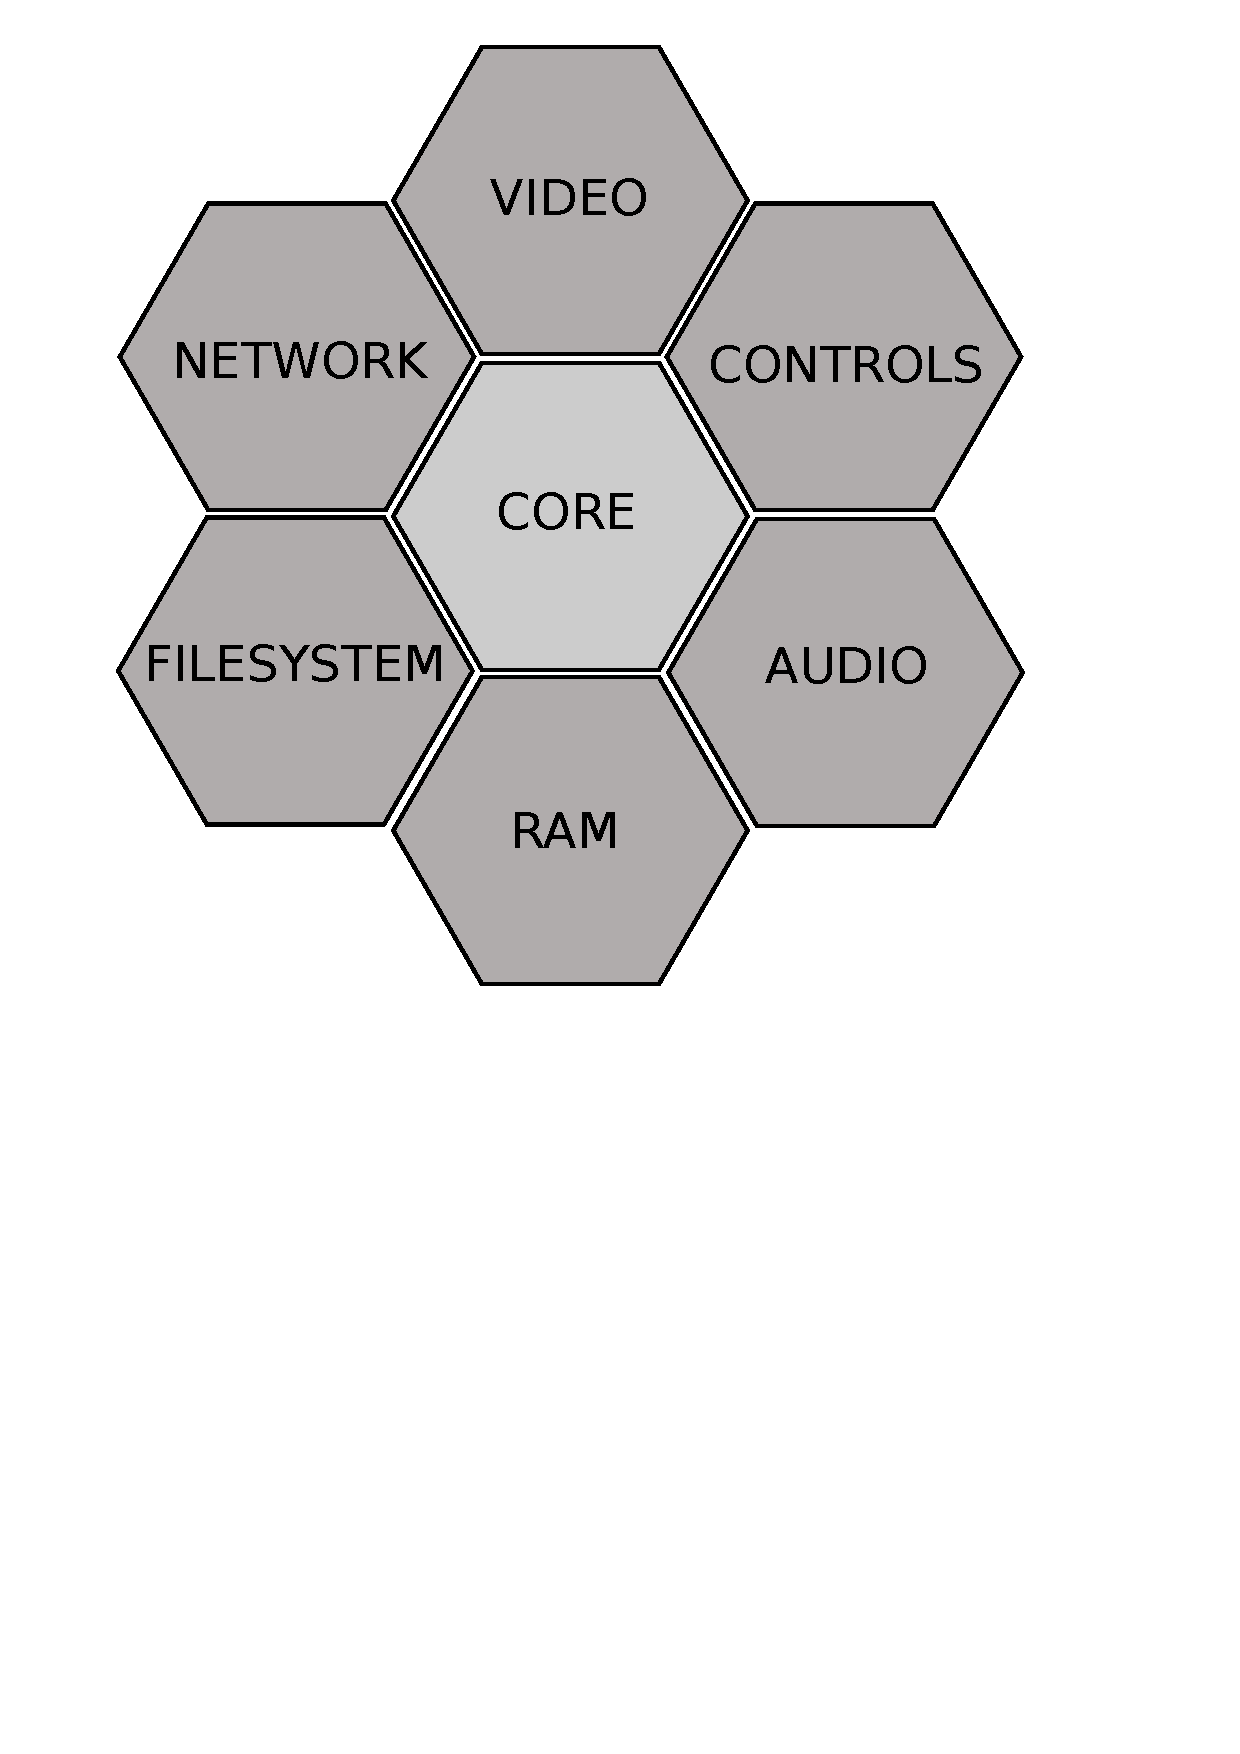
\includegraphics[width=.5\textwidth]{drawings/doom_arch.pdf}
\caption{Doom kernel and its I/O platform-dependent systems.}
\end{figure}
\par
In the case of the video system, it would be using the VGA on MS-DOS but \cw{NSWindow} API on \NeXT. A naive implementation would have required a layer of indirection to dispatch each I/O call. There was a better solution which leveraged C's linking step.\\
\par
 While building a C program, all compilation units (\cw{.c} files) are compiled independently. At the end of the compilation step, all \cw{.c} have been transformed into object (\cw{.o}) files. Object files maybe calling each others but because they were created independently, they have "holes" called "Unresolved Symbols".\\
\par
 To generate an executable, all objects are given to a linker which will recognize Unresolved Symbols from all objects and patches all holes.\\
 \par
 Taking the example of \cw{s\_sound.c} which is part of the core and looking at \cw{s\_sound.o} this translation unit is found to use function such as \cw{I\_PlaySong} or \cw{I\_StartSound} which are defined in the platform specific sound system. \\
\par
\tcode{s_sound_linker.txt}
\par
After the linker is done, there are no more unresolved symbols. The final executable is ready to run.\\
\par
\drawing{linking}\\




\pagebreak
\drawing{doom_code_arch}{}
\par
In white, the core components. In grey the I/O system which require platform specific code. On DOS these are provided by six extra files: \cw{i\_main.c}, \cw{i\_ibm.c}, \cw{planar.asm}, \cw{i\_ibm\_a.asm}, \cw{i\_sound.c} and, \cw{i\_cyber.c}.\\







\fullimage{Doom_build_NeXTStep.png}
\smallfakedosoutput{dos_compilation2.txt}




\par
\trivia{Notice the prefix one file name. Since C language has no namespace these prefix are also applied to functions names. \cw{I\_} stands for "Implemention specific", \cw{P\_} gameplay, \cw{R\_} is for renderer and so on.}\\

The beauty of this architecture is that once the platform specific systems are written, there is zero overheard to writing code running on multiple platform. Most of the code goes into the kernel and the platform specific code needs not to be touched anymore.\\
\par
\trivia{Because portability was not an afterthought but part of the development process, \doom code layering is never violated. This rigorous design explains partly why \doom has been ported on so many systems. Having to comply with several compiler such as gcc or watcom also make the code more standard compliant and robust.}\\

\section{Diving In!}
Just before finally jumping in, a few quick \cw{cloc} stats just to know what volume to expect. There is twice as much code as in Wolfenstein 3D.\\
\par
\tcode{cloc.txt}
\par
\trivia{\NeXT platform specific were all written in Objective-C: \cw{DRCoord.m}, \cw{VGAView.m}, \cw{Doom\_main.m}, \cw{i\_next.m}, \cw{r\_debug.m},  }\\
\par
\begin{figure}[H]
\centering
  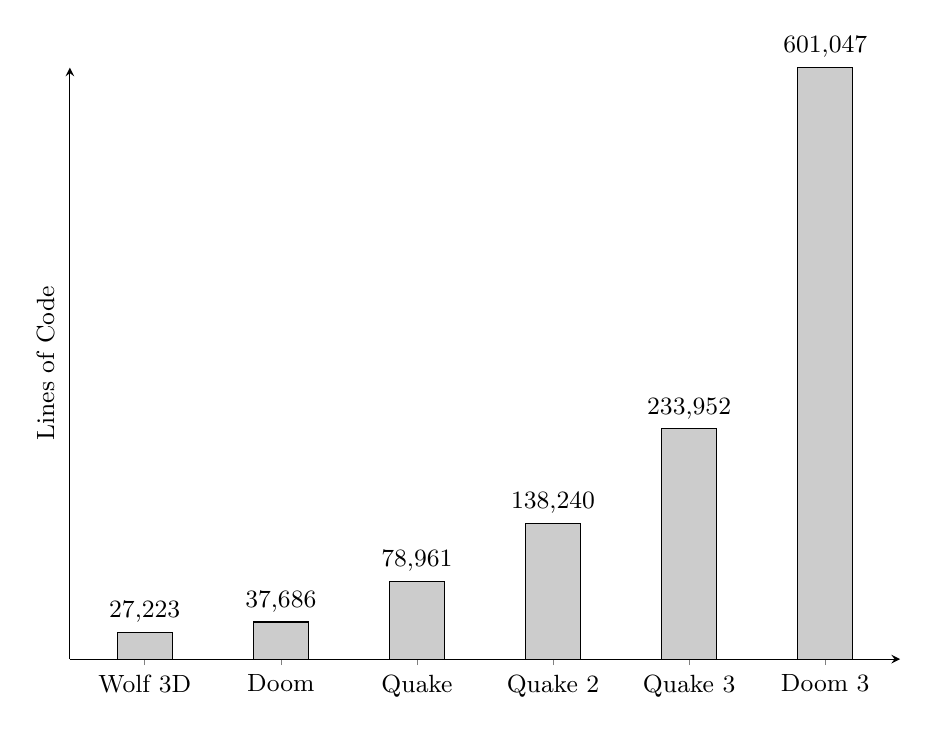
\begin{tikzpicture}[font=\small]
    \begin{axis}[
      width=\textwidth,
      height=0.75\textwidth,
      ybar=0.6\textwidth,
      bar width=20pt,
      ylabel={Lines of Code},
      ymin=0,
      ytick=\empty,
      xtick=data,
      axis x line=bottom,
      axis y line=left,
      enlarge x limits=0.11,
      symbolic x coords={Wolf 3D,Doom,Quake,Quake 2,Quake 3, Doom 3},
      xticklabel style={},
      yticklabel style={},
      nodes near coords={\pgfmathprintnumber[fixed,precision=0]\pgfplotspointmeta}
    ]
      \addplot[fill=black!20,draw=black] coordinates {
        (Wolf 3D,27223)
        (Doom,37686)
        (Quake,78961)
        (Quake 2, 138240)
        (Quake 3, 233952)
        (Doom 3, 601047)
      };
    \end{axis}
   \end{tikzpicture} 
   \caption{Lines of code from id Software game engines.}
 \end{figure}

\par
 \begin{figure}[H]
\centering  
\begin{tabularx}{\textwidth}{ L{0.22} | C{0.39} | C{0.39} }
  \toprule
  \textbf{System} & \textbf{DOS Implementation} & \textbf{NeXT Implementation}\\
  \toprule 
    Video System & VGA & NSWindow/libinterceptor\\
    Audio System & DMX & Not Implemented\\
    Control System & DMPI Interrupts & NSWindow/NXEvent \\
    File  System & Direct & BigEndian converter\\
    Network System & Direct interrupt & BSD socket \\
    RAM System & greedy malloc & tight 4 MiB malloc\\
   \toprule
\end{tabularx}
\caption{Platform code specific.}
\end{figure}

\par


The \cw{main} function can be found in \cw{i\_main.c} translation unit\footnote{On \NeXT there is no \cw{main} function since it is part of the window system. \cw{D\_DoomMain} is directly called from there.}. It jumps right into \cw{D\_DoomMain} which initialize all systems in order.\\
\par
\ccode{main_loop.c}
\pagebreak

The function calls match exactly what players could see in the DOS prompt upong starting the game.\\
\par
\fakedosoutput{doom_dos_start.txt}
% InitTextures 
% InitFlats........  
% InitSprites 
% InitColormaps 
% R_InitData 
% R_InitPointToAngle 
% R_InitTables 
% R_InitPlanes 
% R_InitLightTables 
% R_InitSkyMaP 
% R_InitTranslationsTables 
\par
\fixme{Startup screen is inacurate. Trivia about dot? Due to textures loading from S\_START to S\_END.}

\section{Fixed time steps}
Peeking inside \cw{D\_DoomLoop} reveals a pretty standard loop where the world is updated and then rendered to the audio and video output.\\
\par
\ccode{doomloop.c}
The method \cw{TryRunTics} will immediately catch the eye of an experience game developer.\\
\par
\ccode{TryRunTics.c}
\par
\doom engine uses fixed time step and runs at 35Hz. Under this architecture, the game renders as fast as possible. However before rendition occurs, the world is updated in small fixed size timeslice increment. In the case of \doom, a timeslice is 1/35\ts{th} of a second which is the equivalent of 28ms.\\
\par
\drawing{fixed}{}
\par
This design choice would end up being controversial. One one side it solved the issue of recording a game session and being able to playback on any machine without desync. It also enabled network play and multiscreen play. On the other side, it meant that no matter how fast the renderer could run, the game would only update at 35Hz which would cap the next generation based on Pentium CPUs.\\
\par



\section{Game thread/Sound thread}
The second interesting thing in \cw{D\_DoomLoop} is \cw{S\_UpdateSounds} which give a clue on how sound is done. MS-DOS did not support process or thread. Yet video and audio must happen in parallel. As a result, the audio system was interrupt based. This is explained in detail in the audio section on page \pageref{dmx_section}\\
\drawing{three_systems}{}
\trivia{Notice the audio system is also in charge of generating heartbeat which \doom uses to pace itself and run at 35Hz.}







\section{Fixed arithemetic}
Before digging further inside the internals of the engine, a few words on how \doom performed mathematics. With floating points unavailable, the engine was forced to do all calculations requiring fraction tracking using fixed point.\\
\par
Conveniently, there is only one type of fixed point in the codebase which is \cw{16:16}.\\
\par

\ccode{fixed_t.c}{}
\par
As a quick recap, under normal operations, a 32-bit \cw{int} is encoded as follows.\\
\par
\begin{figure}[H]
 \centering
  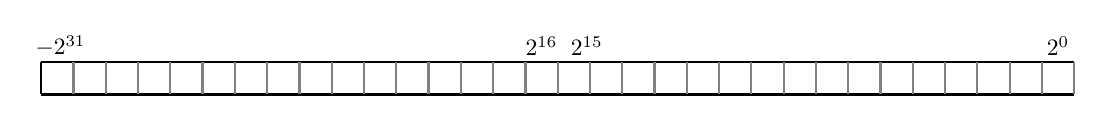
\begin{tikzpicture}[scale=0.41, every node/.style={scale=0.85}]


\colorlet{LighterMark}{black!50}

% Dark marks
\draw[thick,black] (0,0) -- (32,0);
\draw[thick,black] (0,1) -- (32,1);

\draw[thick,black] (0,1) -- (0,0);
\draw[thick,black] (32,1) -- (32,0);

% Light marks
\foreach \i in {1,...,32}
{
     \draw[thick,LighterMark] (\i,1) -- (\i,0);
}


% Labels      
\node[] at (31+0.5  ,1.5){$2^{0}$  }  ;      
\node[] at (16.5+0.4,1.5){$2^{15}$  }  ;     
\node[] at (15+0.5  ,1.5){$2^{16}$  }  ;     
\node[] at (00+0.6  ,1.5){$-2^{31}$  }  ;     


\end{tikzpicture}

 \caption{32-bit signed two complement encoded integer.} \label{fig:mips}
\end{figure}

\begin{figure}[H]
 \centering
  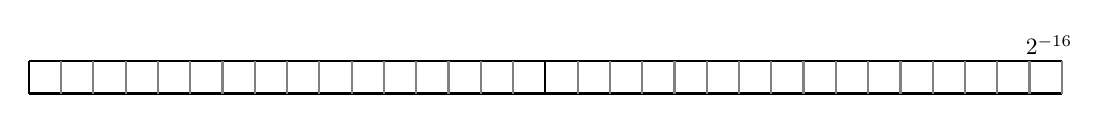
\begin{tikzpicture}[scale=0.41, every node/.style={scale=0.85}]


\colorlet{LighterMark}{black!50}

% Dark marks
\draw[thick,black] (0,0) -- (32,0);
\draw[thick,black] (0,1) -- (32,1);

\draw[thick,black] (0,1) -- (0,0);

\draw[thick,black] (32,1) -- (32,0);

% Light marks
\foreach \i in {1,...,32}
{
     \draw[thick,LighterMark] (\i,1) -- (\i,0);
}

\draw[thick,black] (16,1) -- (16,0);

% Labels      
\node[] at (31+0.6,1.5){$2^{-16}$  }  ;    
     




\end{tikzpicture}

 \caption{Fixed point layout 16:16 (16 bits for the integer part and 16 bits for the fractional part).} \label{fig:mips}
\end{figure}

\pagebreak
Bla
\pagebreak

